% Possíveis TODO
% - expandir nas equacoes xx yy
\documentclass[a4paper,titlepage]{article}
\usepackage[utf8]{inputenc}
\usepackage[T1]{fontenc}
\usepackage[brazil]{babel}
% setspace - \doublespace \onehalfspace
% fullpage - ?? 

\usepackage{verbatim}
\usepackage{url}
\usepackage{hyperref}
\usepackage{graphicx}
\usepackage[bf]{subfigure}
\usepackage[bf]{caption}
\usepackage{amsmath,amssymb}
\usepackage{algorithm,algorithmic}
\usepackage{mathtools,empheq}
\usepackage{macrosfabbri-basic}
\usepackage{xcolor}
\usepackage{ulem}

% ------------------------------------------------------------------------------
% Paper draft Comments and TODO's
%
% You have two versions of the macro
% \draftnote{My note}. The first version puts notes (e.g. My note in the example)
% into the margin of your document. The second formats the note as nothing. You
% 'comment out' the version of the macro you don't want (using a % at the
% beginning of the line).
\newcommand{\draftnote}[1]{\marginpar{\tiny\raggedright\textsf{\textcolor{blue}{\hspace{0pt}#1}}}}
%\newcommand{\draftnote}[1]{}
%
% This one is just for the comments for in-line text.
\newcommand{\indraftnote}[1]{\textcolor{blue}{\texttt{\footnotesize [#1]}}}
\newcommand{\todo}[1]{\indraftnote{todo: #1}} % Este  "a fazer" é para eu não esquecer
\newcommand{\juliana}[1]{\textcolor{red}{#1}}


\begin{document}

\begin{titlepage}
\renewcommand{\title}{%
  {\LARGE Revisão Comentada de Artigo}\\
  \mbox{Barycentric Subspace Analysis on Manifolds}%
}
\renewcommand{\author}{Juliana Santos Barcellos Chagas Ventura\\ Gabriel Andrade}
\renewcommand{\date}{\today}
\newcommand{\info}{%
  \raisebox{4pt}[-4pt]{%
  \includegraphics[height=1.3cm]{figs/logo-iprj.png} 
  \hspace{0.1in}
  }\\

  Instituto Politécnico -- IPRJ\\
  Universidade do Estado do Rio de Janeiro\\[2em]
  
  \includegraphics[height=1.3cm]{figs/logo-ppgmc.png}\\
  Programa de Pós Graduação em Modelagem Computacional\\
  Disciplina de Variedades Diferenciáveis\\
  prof. Ricardo Fabbri\\[1em]

  Nova Friburgo, \date\\[1.5cm]
}

%% Abstand zwischen oberem Blattrand und Titel.
\newlength{\topToTitle} 
\setlength{\topToTitle}{0pt}

%% Abstand zwischen linkem Blattrand und Titel.
\newlength{\leftToTitle} 
\setlength{\leftToTitle}{-60pt}

%% Abstand zwischen Titel und Info-Feld.
\newlength{\titleToInfo} 
\setlength{\titleToInfo}{9.5cm}

%% \myTextWidth erhoehen, um Info-Feld weiter nach Rechts zu schieben.
\newlength{\myTextWidth}
\setlength{\myTextWidth}{\textwidth}
\advance\myTextWidth by 1cm


\thispagestyle{empty}
\vspace*{\topToTitle}
\begin{minipage}{\myTextWidth}
  \sffamily
  \hspace*{\leftToTitle}\begin{minipage}{11cm}
    \Large\textbf{Trabalho final}\\[1.5cm]
    \title\\[1.5cm]
    \author
  \end{minipage}\\

  %% \enlargethispage{} um ggfs. Titel und Info-Feld weiter
  %% auseinanderziehen zu koennen.
  \vspace*{\titleToInfo}

  \begin{minipage}{\textwidth}
    \flushright
    \info
  \end{minipage}
\end{minipage}%
\end{titlepage}


\section{Preliminares}

Este trabalho consiste em expandir o artigo~\cite{Pennec:AnnStat:2018},
cuja primeira página está reproduzida na Figura~\ref{fig:paper:page1}.
O presente texto é uma versão comentada do artigo,
expandindo o máximo possível os conceitos ligados a Variedades Diferenciáveis.
Desta forma, o presente texto é um super-conjunto do referido artigo.
Ele contém todo o artigo, possivelmente em forma de recortes, com expansões e
comentários, e conexões com outros conceitos.

\begin{figure}
\centering
\frame{\includegraphics[width=0.8\linewidth]{figs/pennec2018-page1.png}}
\caption{% 
Primeira página do artigo sendo revisado. Para baixar, foi necessario o Scihub
pois o portal da CAPES nao continha este periodico apos 2017.
}\label{fig:paper:page1}
\end{figure}

Será utilizada uma mistura de línguas nesta revisão, sendo o inglês preferido
sempre que possível. Sendo assim, não teremos o trabalho de traduzir do inglês
algumas construções básicas do \LaTeX\ como \emph{Theorem} ou
\emph{Definition}.


\section{Tabela de Notação}

This section has a summary of the notation used in the paper, 
mapped to the master notation.

\section{Commented and Expanded Abstract}

Aqui devemos comentar o abstract. Neste caso, escolhemos por comentar
cada parágrafo. Nesta seção, devemos procurar usar linguagem e observações mais
gerais, como se fosse um resumo expandido. Abaixo segue um screen shot do primeiro paragrafo.

{
\vspace{1em}
\frame{\includegraphics[width=0.8\linewidth]{figs/pennec2018-abstract-paragraph1.png}}
\vspace{1em}
}

Aqui o autor comenta que irá realizar uma extensão de PCA para Variedades
Riemannianas.

Variedades Riemannianas podem surgir, por exemplo, no contexto de \emph{data science}, de um conjunto de dados
provenientes de fenômenos não-lineares, em que os dados possuem uma estrutura de
similaridade ou métrica.

\todo{O que seria um espaço geodésico que não é Riemanniano?}

{
\vspace{1em}
\frame{\includegraphics[width=0.8\linewidth]{figs/pennec2018-abstract-paragraph2.png}}
\vspace{1em}
}

\section{Commented and Expanded Section 1: Introduction}

{
\vspace{1em}
\frame{\includegraphics[width=0.8\linewidth]{figs/pennec2018-p1-paragraph1-intro.png}}
\vspace{1em}
}

Em poucas palavras, o PCA em espaços lineares (afim) pode ser definido
como o menor sub-espaço afim ($\mathbb R^n$ transladado) que contém os dados;
caso uma dimensão $n$ seja especificada, então o PCA de um conjunto é 
o menor sub-espaço afim de dimensão $k$ que capture a máxima variância dos dados
com $k$ dimensões. Se $k$ for maior que a dimensão do espaço que contém os dados
sem erro, então o PCA pode ser calculado sem perda. Se $k$ for menor que esse
valor, então o PCA vai conter perda. Conforme sabemos de Variedades
Diferenciáveis, muitos conjuntos de dados amostrados de fenômenos não-lineares,
por exemplo os provenientes de variedades diferenciáveis ou \emph{manifolds},
não são descritíveis globalmente por um único sistema de coordenadas de dimensão
míninima ou intrínseca. Logo, o PCA na maioria dos casos não-lineares incorre no
problema de ineficiência, pois muitos fenômenos não-lineares de forma global
com um único sistema de coordenadas cartesiano.

Note that it is possible to represent non-manifold areas of a nonlinear dataset
using PCA, it just won't be the minimum linear space or tangent space, but might
have to have larger dimensions. For instance, a 2D cross x might need a 2D space
to be represented using extrinsic coordinates $\mathbb R^2$ (the plane
containing the $x$). So PCA is useful for non-manifold data; it just might not
be the most efficient one. But if one considers it can reduce from 10000
dimensions (say the $x$ represented by a $100\times100$ image) to 2 is already a
the biggest step in terms of compression.

PCA being ``nested'' means that the PCA subspace of dimension $k$ contains the
PCA subspace of dimension $k-1$. That is, the dimensions of the PCA are ordered,
so that if PCA has dimension $n$ then the lower dimensional subspaces that are
``best fit'' for the data are simply the same PCA subspace, but with the lower
dimension removed (the dimension along which the data has least variance). 
 
 \draftnote{As partes que eu, Juliana, acrescentar colocarei em vermelho para facilitar pra mim. Depois tirarei.}
 \juliana{No caso euclidiano, na abordagem \textit{forward} inicia-se com a média da amostra para encontrar a primeira autodireção da matriz de covariância, que determina a reta que melhor ajusta os dados. O processo segue de forma iterativa resultando numa sequência de espaços afins que melhor ajustam os dados, "nested" em ordem crescente de dimensão. Já na abordagem \textit{backward}, inicia-se com o melhor espaço afim de dimensão r que ajusta os dados. Dentro dele procura-se o melhor espaço afim de ajuste de dimensão r-1, etc. O que também resulta em uma sequência dos melhores espaços de ajuste, indexados pela dimensão. pelo teorema de Pitágoras, ambas as abordagens resultam na mesma sequência de espaços afins. Porém, em espaços não euclidianos a igualdade das sequências não se verifica. (DAMON, J. MARRON, J. S. 2013) }
 
{
\vspace{1em}
\frame{\includegraphics[width=0.8\linewidth]{figs/pennec2018-p1-paragraph2-intro.png}}
\vspace{1em}
}
\draftnote{Revisar aqui a media de Fréchet e também rapidamente o Karcher mean}
\draftnote{Gabriel's comment}
\\
Neste trecho, o autor nos informa as condições as quais devemos ter para que tal generalização seja feita. Uma delas é que definamos um equivalente a subespaços afins em termos de variedades. Primeiramente o que é um espaço afim? Um espaço afim é definido informalmente como um espaço que não possui uma origem definida \draftnote{Notas do Gabriel: Por favor me expliquem melhor para que eu possa explicar corretamente}.
\\
\juliana{Seja $V$ um espaço vetorial. $W \subset V$ é um subespaço afim de V se existir um vetor $w_0 \in V$ e um subespaço vetorial $V_0 \subset V$ tal que $$W=\{w_0 +v ; v \in V_0 \}.$$}
\juliana{Se $V=\mathbb{R}^2$ ou $V=\mathbb{R}^3$. O subespaço afim W é o subconjunto obtido da translação do subespaço vetorial $V_0$ (que por definição passa pela origem (0,0) ou (0,0,0), respectivamente) de modo que a origem esteja em $w_0$, ou seja, W é um subconjunto "paralelo'' a $V_0$ que passa pelo ponto $w_0$.}

Pode-se dizer também, segundo o autor, que para um espaço de dimensão zero, ou seja, um espaço discreto \draftnote{Gabriel's comment: link de onde tirei isso \url{https://encyclopediaofmath.org/wiki/Zero-dimensional_space}} uma abordagem com o uso da média de Fréchet no conjunto da minima da variança é naturalmente pensada quando aborda-se o problema em termos de variedades. A média de Fréchet é uma generalização aos centróides, onde é encontrado um ponto em um conjunto de pontos que possa melhor representar a tendência dos mesmos no grupo. 
Em termos de variedades, supondo que tenhamos uma nuvem de pontos discretos dentro de um espaço de variedades, o uso da média de Fréchet nos ajudaria a encontrar a tendencia desta nuvem, proporcionando uma melhor escolha de componentes pela PCA. \draftnote{Gabriel's comment: Foi pelo menos o que eu a principio entendi deste trecho}
\\
\juliana{A média de Fréchet é uma generalização da média aritmética em espaços métricos abstratos e, em geral, não é única (Ginestet, Simmons, Kolaczyk, 2012).}
\\
\juliana{Um ponto $\mu$ em um espaço métrico \textbf{M} com função distância $\rho$ é chamado de média de Fréchet da variável aleatória $X$ em \textbf{M} se satisfaz
$$\mu=arg \min \limits_{x \in M} E[\rho(x,X)^2].$$
Se \textbf{M} é uma variedade riemanniana, ela é localmente homeomorfa a um espaço euclidiano e as distribuições limites para as médias de Fréchet das amostras são, em geral, gaussianas; fenômeno semelhante ao das médias euclidianas (LE, H. 2015). A curvatura seccional de uma superfície é uma generalização da curvatura gaussiana; assim, se a curvatura gaussiana é negativa, então a curvatura seccional também é. Portanto, em uma variedade Riemanniana completa, simplesmente conexa e de curvatura seccional não-positiva a média de Fréchet é única (POLANÍA, 2014).}
\draftnote{Juliana's comment:Explicar melhor}


\section{Commented and Expanded Section 2: Riemannian geometry}

\begin{center}
\fbox{\parbox[c]{11cm}{In statistics, directional data occupy a place of
choice [Dryden (2005), Huckemann and Ziezold (2006)]. Hyperbolic spaces are
also the simplest models of negatively curved spaces which model the space of
isotropic Gaussian parameters with the Fisher–Rao metric in information geome-
try [Costa, Santos and Strapasson (2015)]. As nonflat constant curvature spaces,
both spherical and hyperbolic spaces are now considered in manifold learning for
embedding data [Wilson et al. (2014)]. Thus, they are ideal examples to illustrate the theory throughout this paper.}}
\end{center}

Neste trecho, o autor nos revela neste parágrafo que em termos de simplicidade, ele escolhe duas abordagens que são as "dados direcionais'' e os espaços hiperbólicos. Os chamados dados direcionais se referem a uma formulação mais recente da estatística conhecido como estatística direcional. Nessa formulação os dados são tratados com suas direções, eixos e rotações. Mais tarde, com as figuras, veremos que ele utiliza os dados da PCA em uma distribuição circular.\draftnote{Gabriel's notes: checar se está correto e reescrever. Preciso entender melhor este processo. Uma reunião talvez...} 
\\
\juliana{Os espaços esférico e hiperbólico são exemplos de espaços pseudo-euclidianos, isto é, espaços cujas dimensões são caracterizadas por autovalores negativos e a distância quadrada entre objetos tem componentes positivos e negativos que são somados para fornecer a distância total. Espaços pseudo-euclidianos não são métricos, o que dificulta calcular corretamente propriedades geométricas. Uma alternativa é imergir os dados em uma variedade curva, que é um espaço métrico, mas não euclidiano (WILSON, \textit{et all}, 2014).}

Os espaços hiperbólicos são escolhidos por serem espaços homogêneos onde a curvatura do espaço é a curvatura do espaço seccionado; \juliana{ela é constante e negativa. Já a curvatura dos espaços esféricos é constante e positiva}. \sout{Uma comparação com o espaço euclidiano, enquanto o simples é utilizando um triângulo construído no espaço euclidiano e no espaço hiperbólico, no espaço euclidiano, a soma dos ângulos "S=180º" no hiperbólico "S<180º''.} \draftnote{Juliana's comment: a parte riscada achei desnecessária. O que acha?}

\begin{center}
\fbox{\parbox[c]{11cm}{\textit{Tools for computing on Riemannian manifolds.} We consider a differential manifold M endowed with a smooth scalar product  $\langle | \rangle$ called the Riemannian metric on each tangent space $T_x M$ at point x of M. In a chart, the metric is specified by the dot product of the tangent vector to the coordinate curves: $gij (x) = \langle \partial i | \partial j \rangle_{x}$ . The Riemannian distance between two points is the infimum of the length of the curves joining these points. Geodesics, which are critical points of the energy functional, are parametrized by arc-length in addition to optimizing the length. We assume here that the manifold is geodesically complete, that is, the definition domain of all geodesics can be extended to $\mathbb{R}$. This means that the manifold has no boundary nor any singular point that we can reach in a finite time. As an important consequence, the Hopf–Rinow–De Rham theorem states that there always exists at least one minimizing geodesic between any two points of the manifold (i.e., whose length is the distance between the two points).}}
\end{center}

Neste trecho o autor começa a nos mostrar o ferramental usado para o artigo. Primeiramente ele deifine uma variedade $M$ com um produto escalar suave, conhecido como métrica Riemmaniana no espaço tangente $T_{x}M$ em um ponto $x$ de $M$ e em seguida ele constrói uma função $g(x)$ tal que $g_{ij}(x)=\langle \partial_i | \partial_j \rangle $. Isso significa que $g_{ij}(x)=||\partial_i||,i=j$, $g_{ij}(x)=\sum (\partial_i \partial_j)^2,i\neq j$, o que representa a derivada direcional \draftnote{Gabriel: Verificar se isso faz sentido}. Ele então, a partir dessa disso, constrói uma geodésica parametrizando pelos ótimos de $g$ e, como ele assume que esta variedade é geodesicamente completa, ele consegue atribuir uma correlção da variedade ao espaço $\mathbb{R}$ chegando a condlusão que a variedade não possui nem ponto de singularidade nem contorno que possa-se chegar em um tempo fnito e, por fim, que o Teorema de Hopf-Rinow-De Rham é satisfeito. \draftnote{Gabriel: Escrever melhor essa parte}

\begin{center}
\fbox{\parbox[c]{11cm}{DEFINITION 1 ((k+1)-pointed/punctured Riemannian manifold). 
\\
\textit{Let ${x_0,...,x_k} \in \mathcal{M}^{k+1}$ be a set of $k + 1$ reference points in the n-dimensional Riemannian manifold $\mathcal{M}$ and $C(x_0,...,x_k) = \bigcup_{i=0}^{k} C(x_i)$ be the union of the cut loci of these points. We call the object consisting of the smooth manifold $\mathcal{M}$ and the $k + 1$ reference points a $(k + 1)$-pointed manifold. Likewise, we call the submanifold $\mathcal{M}^{*}(x_0,...,x_k) = \mathcal{M} \ C(x_0,...,x_k)$ of the non-cut points of the $k + 1$ reference points a $(k + 1)$-punctured manifold.}}}
\end{center}

\begin{center}
\fbox{\parbox[c]{11cm}{On $\mathcal{M}{*}(x_0,...,x_k)$, the distance to the points ${x0,...,xk}$ is smooth. The Riemannian log function $\vec{x x_i} = \log_x(x_i)$ is also well defined for all the points of $\mathcal{M}{*}(x_0,...,x_k)$. Since the cut locus of each point is closed and has null measure, the punctured manifold $\mathcal{M}{*}(x_0,...,x_k)$ is open and dense in $\mathcal{M}$, which means that it is a submanifold of $\mathcal{M}$. However, this submanifold is not necessarily connected.
For instance in the flat torus $(S_1)^n$, the cut-locus of $k + 1 \leq n$ points divides the torus into kn disconnected cells.}}
\end{center}

Nesta seção

\vspace{1em}
\frame{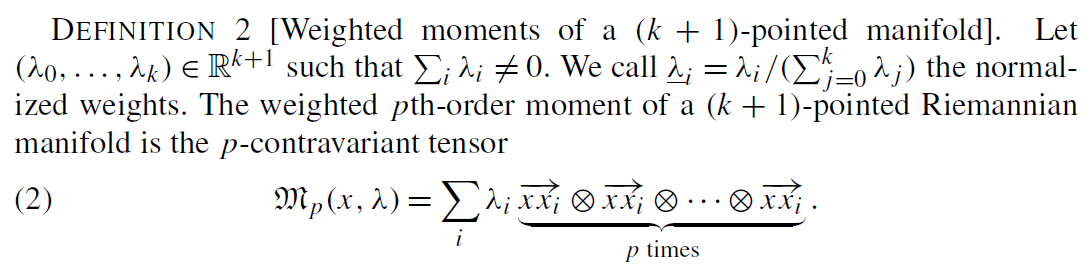
\includegraphics[width=0.95\linewidth]{figs/pennec2018-def2.PNG}}
\vspace{1em}

\begin{center}
 \fbox{\parbox[c]{11cm}{DEFINITION 3 (Affinely independent points). A set of $k + 1$ points ${x_0,...,x_k}$ is affinely independent if no point is in the cut-locus of another and if all the sets of $k$ vectors ${\log_{x_i}
(xj)}_{0\leq j\neq i \leq k} \in T_{x_i}\mathcal{M}^k$ are linearly independent.}}
\end{center}


\section{Commented and Expanded Section 3: Exponential Barycentric Subspaces
(EBS) and affine spans}

\vspace{1em}
\frame{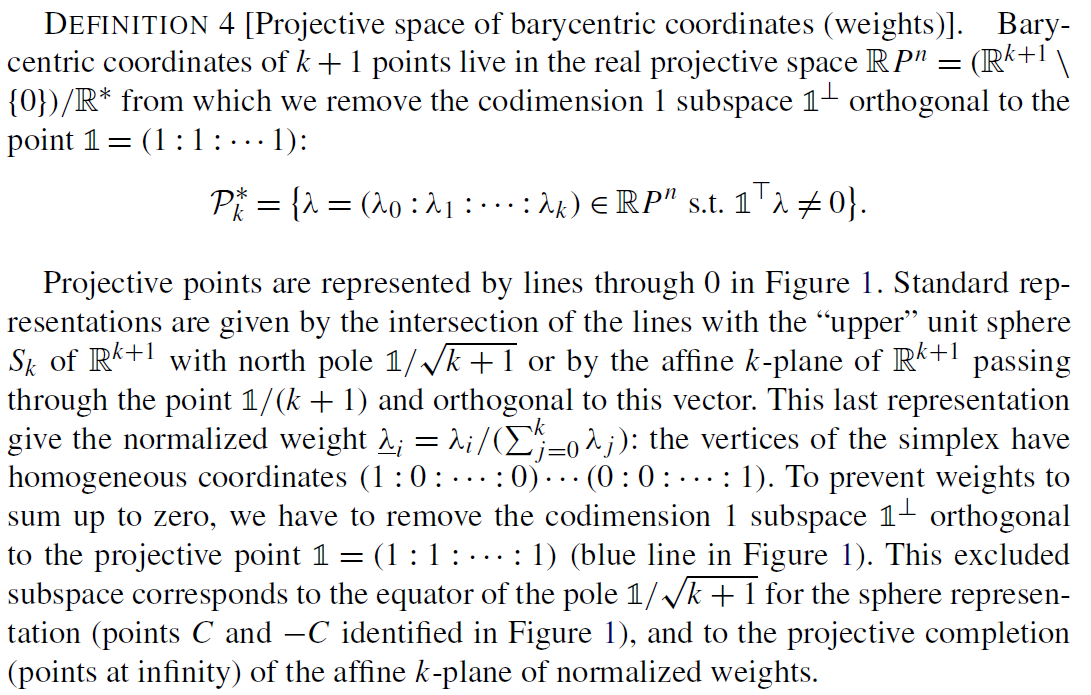
\includegraphics[width=1\linewidth]{figs/pennec2018-def4.PNG}}
\vspace{1em}


\section{Commented and Expanded Section 4: Fréchet/Karcher barycentric subspaces}

{
\vspace{1em}
\frame{\includegraphics[width=0.8\linewidth]{figs/pennec2018-p18-fig2.png}}
\vspace{1em}
}

\todo{explicar cada figura do paper com proprias palavras e de forma expandida}

\section{Commented and Expanded Section 5: Properties of the barycentric
subspaces}

\section{Commented and Expanded Section 6: Barycentric subspace analysis}

\section{Commented and Expanded Section 7: Discussion}

\section{Commented and Expanded Appendix: Proof of Theorem 8}
Nesta seção o autor nos provém primeiramente com uma função que pega e leva de $x  a y \notin C(x)$ em respeito ao tempo e ele também nos informa que revertendo o tempo ao longo da geodésica, tem-se $\gamma_{(x,\overrightarrow{xy})}(t)=\gamma_{(y,\overrightarrow{yx})}(1-t)$, e ele também diz que em  $\dot{\gamma_{(x,\overrightarrow{xy})}}(1)=\dot{\gamma_{(y,\overrightarrow{yx})}}(0)=-\overrightarrow{yx}$. Isto que o autor faz em um espaço geodésico é similar a uma abordagem em uma parametrização em um espaço euclidiano $x(t)=x_{0}t+(1-t)x_{1}$ e pelo que pode-se entender $\overrightarrow{xy}$ é o vetor distância de $x$ a $y$, portanto faz sentido que $\overrightarrow{xy}=-\overrightarrow{yx}$. Então ele define que $\gamma_{(x,\overrightarrow{xy})}(t)=exp_{x}(t \overrightarrow{xy})$, temos $\overrightarrow{yx}=-D exp_{x}|_{\overrightarrow{xy}}\overrightarrow{xy}$\draftnote{Gabriel's note: Por favor expandir isso!}. Pelo fim do parágrafo é definido que $(D exp_{x}|_{\overrightarrow{xy}}\overrightarrow{xy})D log_{x}|_{y} = Id$ pelo fato de $exp_{x}(log_{x}(y))=y$ e finalmente ele considera que se tanto $Dexp_{x}$ quanto $Dlog_{x}$ possuírem o posto aquivalente ao expaço quociente da variedade com o domínio em x, podemos criar uma função inversa como descrito na equação (16). No segundo parágrafo, tendo as funções definidas ele considera uma bola aberta geodésica $B(x_0,\xsi)$ e se for construído um domínio $D_{\xsi}=M \\ C(B(x_0,\xsi)$ em q $log_{x}(y)$ seja suave e bem definida na bola e para todo y em D, a simetria é preservada, portanto (16) pode ser reescrito como (17) 

%\section{Commented and Expanded Supplementary Material}

Teste


\bibliographystyle{ieeetr}
\bibliography{refs}
%bib/edge-linking,bib/deformable,bib/medical,bib/graphics,bib/texture,bib/imaging,bib/tracking,bib/shape-papers,bib/bib-header,bib/video,bib/math-books,bib/math,bib/psych-books,bib/metric,bib/edge,bib/leymarie_pami_scaffold,bib/vision-books,bib/vision,bib/nn-search,bib/multidimscaling,bib/psychophysics,bib/indexing,bib/segmentation,bib/image-databases,bib/shape-matching,bib/neuro,bib/skeleton,bib/skeleton2D,bib/aspect-graphs,bib/recognition,bib/surface-networks,bib/ridge,bib/proceedings,bib/perceptual-grouping,bib/continuation,bib/graph-matching-2,bib/cooper}
%DAMON, J. and MARRON, J. S. (2013). Backwards principal component analysis and principal nested relations. J. Math. Imaging Vision 50 107–114. MR3233137
%\input{paper.bbl}
% Le, Huiling. “A DIFFUSION PROCESS ASSOCIATED WITH FRÉCHET MEANS.” The Annals of Applied Probability, vol. 25, no. 6, 2015, pp. 3033–3046., www.jstor.org/stable/24521650. Accessed 30 June 2021.
%WILSON, R. C., HANCOCK, E. R., PEKALSKA, E. and DUIN, R. P. W. (2014). Spherical and hyperbolic embeddings of data. IEEE Trans. Pattern Anal. Mach. Intell. 36 2255–2269.

% Assinaturas:
%\newpage
%\ \\\vspace{7cm}
%\center $\overline{\ \ \ Ricardo\ Fabbri\ \ \ }$
%\ \\\vspace{4cm}
%\center $\overline{\ \ \ Luciano\ da\ Fontoura\ Costa\ \ \ }$
\end{document}
